So that the electronics may work as intended, power-supplies are required. Constant DC voltages with a high current-output must be generated to power the components of the impedance-sensing system. \par

The DC value of these power-supplies depend on the requirements of the chips present in the PCB. For this system, power-supplies of 5V, 3.3V, 2.5V, 1.8V, and 1.65V must be created. The general scheme devised for the power-supplies is that a low-voltage battery of 2.5V would be connected to the PCB. This voltage being lower than some of the power-supplies, a Boost step-up converter is required to create a 5V voltage. The other supplies would be stepped-down from this 5V using linear regulators. The 1.8V supply is used to power the MCU (see \autoref{sec:MCU}) of the system. The MCU needs to be active whenever the system is powered on since it enables the other power-supplies. The whole power-management scheme is shown in \autoref{fig:PowerManagement} \par
\begin{figure}[h]
    \centering
    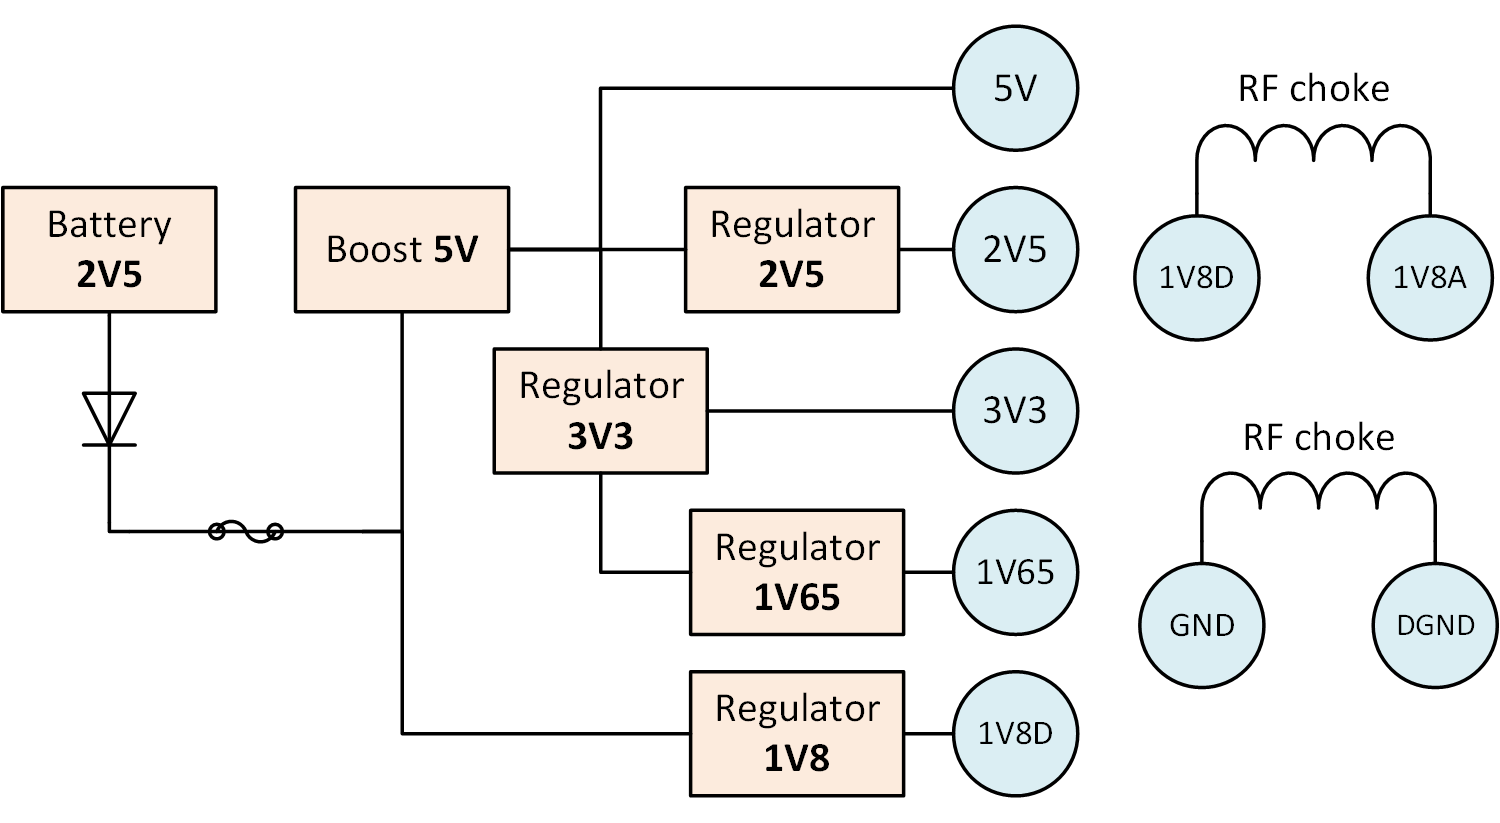
\includegraphics[width=0.9\textwidth]{PowerManagement}
    \caption{Power-management scheme of the impedance-sensing system.}
    \label{fig:PowerManagement}
\end{figure}

Boost converters are adequates supplies for high-power applications since their efficiency is high, upward of 70\%. They do, however, introduce ripples in the system, which increases the noise level at the switching frequency. Adequate filtering is necessary at the converter's output to assure a reference voltage as clean as possible.

Linear regulators are used for the other power-supplies since they demand less power. These types of regulators are precise and linear to the output current, but are not efficient since the regulation voltage (i.e. the subtracted voltage from the input magnitude) is simply wasted as heat and dissipated in the chip. \par

Reference voltages can also be created using a voltage divider and a buffer. Those references, however, cannot provide much power to the load since they are limited by the current output of the buffer. \par

Digital circuitry creates lots of high frequency noise when switching between their binary voltages (0s and 1s), which can introduce high-frequency switching noise in the voltage reference. In order to not contaminate the reference voltages, different planes sharing the same voltages are used. Inductor chokes can be used to reduce the noise shared between reference planes of identical voltages, by linking their DC voltage but blocking the high-frequency components.   \par